\documentclass[a4paper,11pt]{article}

\usepackage[top=18mm,bottom=22mm,left=18mm,right=18mm]{geometry}
\usepackage{fontspec}
\usepackage{xeCJK}
\setmainfont{Times New Roman}
\setCJKmainfont{Yu Gothic}
\setmonofont{Consolas}
\setCJKmonofont{Yu Gothic}
\usepackage{graphicx}
\usepackage{booktabs}
\usepackage{longtable}
\usepackage{array}
\usepackage{url}
\usepackage{pdflscape}
\usepackage[unicode]{hyperref}
\usepackage{fancyvrb}

\hypersetup{
  colorlinks=true,
  linkcolor=blue,
  urlcolor=blue,
  pdftitle={BWSC2027 Team Operations Manual},
  pdfauthor={Codex}
}

\setlength{\parskip}{0.4em}
\setlength{\parindent}{1em}
\renewcommand{\arraystretch}{1.18}
\Urlmuskip=0mu plus 2mu

\title{BWSC2027 Team Operations Manual}
\author{solar\_ws0129-main}
\date{2026-06-17}

\begin{document}
\maketitle

\section{この文書の目的}

この文書は、和歌山大学ソーラーカーチームのメンバーが、
\textbf{本パッケージを作者不在でも理解し、準備し、運用し、改善できる状態}
になるための引き継ぎ資料である。

対象読者は次のとおりである。

\begin{itemize}
  \item 戦略担当
  \item 伴走車オペレータ
  \item 車両制御・マイコン担当
  \item 実測・同定担当
  \item 新規加入メンバー
\end{itemize}

ゴールは次の 5 点である。

\begin{enumerate}
  \item workspace が何をしているかを理解する
  \item 何が未確定で、何を集める必要があるかを理解する
  \item \path{PowerShell} から各モードを起動・停止できる
  \item \path{live_wifi} を BWSC2027 本番運用へつなげられる
  \item dashboard を見て、正常・異常・次に取るべき行動を判断できる
\end{enumerate}

\section{BWSC2027 の公式前提}

このパッケージは BWSC2027 を想定して整理しているが、
\textbf{大会固有値は必ず公式資料で再確認}すること。

2026年6月17日時点で、公式サイトで確認できる重要事項は次である。

\begin{itemize}
  \item 開催期間: \path{2027-08-22} から \path{2027-08-29}
  \item ルート: \path{Darwin -> Adelaide}
  \item ルート長の目安: 約 \path{3,020 km}
  \item Team Manager's Guide によれば、2027 route notes は \textbf{2027年6月から電子配布予定}
\end{itemize}

公式資料:

\begin{itemize}
  \item Event Regulations: \url{https://worldsolarchallenge.org/2027-event/regulations}
  \item 2027 Event Regulations PDF: \url{https://assets.worldsolarchallenge.org/app/uploads/2026/05/06130905/2027-BWSC-Event-Regulations-V1.0-Published-07052026.pdf}
  \item 2027 Team Manager's Guide PDF: \url{https://assets.worldsolarchallenge.org/app/uploads/2026/05/06130911/2027-BWSC-Team-Managers-Guide-V1-Published-07052026.pdf}
  \item Route Map: \url{https://worldsolarchallenge.org/about-us/route-map}
  \item Dates article: \url{https://worldsolarchallenge.org/latest-news/2027-dates-regulations-announced}
\end{itemize}

重要な注意:

\begin{itemize}
  \item 2027 route notes はまだ repo に入っていない
  \item control stop の最終定義も未反映である
  \item この repo の route / stop / weather の一部は sample である
\end{itemize}

\section{このパッケージが担う役割}

本パッケージは、ソーラーカー戦略運用を次の 3 層で支える。

\subsection{事前準備}

\begin{itemize}
  \item 実測データ整理
  \item 同定
  \item route/profile/map の生成
  \item 天候予報 CSV 取得
  \item 大会全体シミュレーション
\end{itemize}

\subsection{本番ライブ運用}

\begin{itemize}
  \item 車両状態受信
  \item 伴走車状態受信
  \item 天候 API 自動取得
  \item 風予報のオンライン補正
  \item 上位プラン再計画
  \item 下位速度司令 1 Hz 生成
  \item ソーラーカー / 伴走車への指令送信
  \item dashboard 表示
  \item ログ保存
\end{itemize}

\subsection{事後改善}

\begin{itemize}
  \item ログ再解析
  \item map / model 更新
  \item 次回シミュレーション精度向上
\end{itemize}

\section{主要モード}

通常入口:

\begin{itemize}
  \item 実行: \path{.\SolarSim.ps1}
  \item 設定: \path{config/solar/bwsc_2027_demo.yaml}
\end{itemize}

\begin{longtable}{p{0.16\linewidth}p{0.30\linewidth}p{0.36\linewidth}}
\toprule
Mode & 目的 & 主 launch \\
\midrule
\endhead
\path{sim} & 画面付きシミュレーション確認 & \path{launch/solarcar_sim.launch.py} \\
\path{measure} & 実測ログ・地図取得 & \path{launch/solar_measurement.launch.py} \\
\path{live} & ROS topic 直結の本番運用 & \path{launch/solar_race_live.launch.py} \\
\path{live_wifi} & WiFi/UDP 文字列連携付き本番運用 & \path{launch/solar_race_live_wifi.launch.py} \\
\bottomrule
\end{longtable}

最重要コマンド:

\begin{Verbatim}[fontsize=\small]
.\SolarSim.ps1 -Action build
.\SolarSim.ps1 -Action simulate
.\SolarSim.ps1 -Action forecast
.\SolarSim.ps1 -Action identify
.\SolarSim.ps1 -Mode measure -Action up
.\SolarSim.ps1 -Mode live_wifi -Action up
.\SolarSim.ps1 -Mode live_wifi -Action graph
.\SolarSim.ps1 -Mode live_wifi -Action stop
\end{Verbatim}

\section{ディレクトリの見方}

\begin{longtable}{p{0.28\linewidth}p{0.58\linewidth}}
\toprule
パス & 役割 \\
\midrule
\endhead
\path{config/solar/} & 運用設定 \\
\path{launch/} & ROS2 launch \\
\path{mpc_solarcar/} & ROS2 node 本体 \\
\path{dashboard/} & dashboard フロント \\
\path{data/route/} & route waypoint / route profile / speed profile \\
\path{data/weather/} & offline 予報 CSV \\
\path{data/race/} & control stop / drive schedule \\
\path{maps/} & 効率 map / Rint / panel map \\
\path{templates/identification/} & 同定 CSV 雛形 \\
\path{templates/network/} & JSON / systemd / ESP32 雛形 \\
\path{scripts/} & simulate / identify / forecast / sender example / graph export \\
\path{outputs/} & 生成物とログ \\
\path{docs/} & この資料群 \\
\bottomrule
\end{longtable}

\section{主な ROS ノードと役割}

\begin{longtable}{p{0.22\linewidth}p{0.28\linewidth}p{0.20\linewidth}p{0.20\linewidth}}
\toprule
Node & 役割 & 主入力 & 主出力 \\
\midrule
\endhead
\path{mpc_node} & 上位・下位プランナ本体 & forecast, route, battery, vehicle state & \path{/planner/speed_cmd}, \path{/planner/summary} \\
\path{telemetry_text_bridge_node} & UDP JSON と ROS topic の橋渡し & UDP packet, planner topics & vehicle/chase topics, planner UDP \\
\path{weather_fetch_node} & Open-Meteo 予報取得 & chase GPS or fallback lat/lon & raw forecast CSV \\
\path{wind_correction_node} & 風予報のオンライン補正 & raw forecast, route, vehicle/chase wind & corrected forecast CSV, \path{/planner/wind_state} \\
\path{solar_autocal_node} & 走行中の自動校正 & measured power, G POA, speed & calibration state \\
\path{distance_node} & \path{s_km} が無いときの距離積分 & \path{/vehicle/speed_kmh} & \path{/vehicle/s_km} \\
\path{grade_node} & slope 推定 & GPS, altitude & slope 関連 topic \\
\path{speed_command_bridge_node} & planner command を車両側へ再配信 & planner speed / mode & vehicle command \\
\path{dashboard_node} & HTTP dashboard & planner / telemetry topics & \path{http://localhost:8080} \\
\path{logger_node} & CSV logging & 各種 topic & \path{outputs/logs/*.csv} \\
\bottomrule
\end{longtable}

\section{主な offline script}

\begin{longtable}{p{0.36\linewidth}p{0.50\linewidth}}
\toprule
Script & 目的 \\
\midrule
\endhead
\path{scripts/solar_sim.py} & 大会全体シミュレーション \\
\path{scripts/fetch_weather_forecast.py} & forecast CSV 取得 \\
\path{scripts/run_identification_pipeline.py} & 同定一括実行 \\
\path{scripts/build_route_profile_from_gps.py} & GPS から route 再構成 \\
\path{scripts/build_ocv_curve.py} & OCV-SOC カーブ生成 \\
\path{scripts/build_rint_map_from_timeseries.py} & Rint map 生成 \\
\path{scripts/build_pv_maps_from_csv.py} & panel / MPPT map 生成 \\
\path{scripts/fit_vehicle_params.py} & \path{CdA}, \path{Crr}, \path{P_aux} などの再推定 \\
\path{scripts/wifi_vehicle_sender_example.py} & 車両送信例 \\
\path{scripts/wifi_chase_sender_example.py} & 伴走車送信例 \\
\path{scripts/wifi_planner_receiver_example.py} & planner packet 受信確認 \\
\bottomrule
\end{longtable}

\section{現在の repo でできること / 未確定なこと}

\subsection{すでにできること}

\begin{itemize}
  \item \path{PowerShell} から build / simulate / measure / live / \path{live_wifi} / graph を実行できる
  \item \path{live_wifi} で UDP JSON 受信・送信ができる
  \item dashboard が 1 画面で見やすく表示される
  \item 風補正ロジックが live forecast に組み込まれている
  \item sample sender で dry run ができる
  \item PDF 資料が生成できる
\end{itemize}

\subsection{まだ本番投入前に埋める必要があること}

\begin{longtable}{p{0.23\linewidth}p{0.25\linewidth}p{0.38\linewidth}}
\toprule
項目 & 現在の状態 & 最終的に必要なもの \\
\midrule
\endhead
\path{route_waypoints_csv} & sample & 2027 実ルート + 実測補正版 \\
\path{route_profile_csv} & sample & 実測から生成した slope/profile \\
\path{speed_profile_csv} & sample & route notes / 制限速度反映版 \\
\path{forecast_csv} & sample + Open-Meteo & 本番方針を決めた forecast workflow \\
\path{stop_yaml} & sample & 2027 route notes 反映版 \\
\path{drive_schedule_yaml} & 2027 仮版 & 2027 公式条件とチーム運用方針に整合した版 \\
\path{model.*} & 初期値 & 実車同定済み値 \\
\path{maps/*.csv} & 既存ファイルあり & 由来確認済み・最新版 \\
\path{ocv_soc_map} & 空欄 & 必要なら生成、不要なら方針明記 \\
WiFi IP/port & 例示値 & 本番ネットワーク設計確定版 \\
sender program & example のみ & 実センサ読み出し込みの本番版 \\
watchdog 方針 & 文書化のみ & 実装・検証済み \\
\bottomrule
\end{longtable}

\section{BWSC2027 までに集めるべき情報}

\subsection{最重要の不足情報}

2026年6月17日時点で、本番運用に対して最も足りていないものは次である。

\begin{enumerate}
  \item 2027 official route notes
  \item 最終 control stop 情報
  \item 実車の最新同定結果
  \item 本番 sender / receiver の実装
  \item 現地ネットワーク設計
  \item 走行当日の運用ルール
\end{enumerate}

\subsection{収集チェックリスト}

\begin{longtable}{p{0.12\linewidth}p{0.28\linewidth}p{0.22\linewidth}p{0.22\linewidth}}
\toprule
分類 & 集めるもの & ソース & 反映先 \\
\midrule
\endhead
公式 & 2027 Regulations 最終版 & BWSC official & \path{docs/}, 運用手順 \\
公式 & 2027 Team Manager's Guide 最終版 & BWSC official & \path{docs/}, 物流手順 \\
公式 & 2027 Route Notes & BWSC official & \path{data/route/}, \path{data/race/} \\
ルート & waypoint, altitude, road note & 実測 + route notes & \path{route_waypoints_csv}, \path{route_profile_csv} \\
速度制限 & 区間速度制限 & route notes & \path{speed_profile_csv} \\
停止情報 & control stop open/close, dwell & route notes & \path{stop_yaml} \\
車両 & mass, CdA, Crr & coastdown / fit & \path{config/solar/*.yaml} \\
駆動 & drive / regen map & 実機測定 & \path{maps/drive_*}, \path{maps/regen_*} \\
電池 & OCV, Rint, temperature effect & bench / log & \path{maps/}, \path{ocv_soc_map} \\
太陽 & panel eff, MPPT eff & sweep / log & \path{maps/panel_*}, \path{maps/mppt_*} \\
天候 & forecast provider 方針 & チーム運用判断 & \path{live.weather.*} \\
風 & wind tuning parameter & dry run / log & \path{live.wind_model.*} \\
通信 & planner PC / solar Pi / chase Pi IP & チーム設計 & \path{live.wifi_bridge.*} \\
通信 & JSON field mapping & firmware / Pi 実装 & sender / receiver program \\
安全 & comm lost 時の速度方針 & チーム運用判断 & firmware と手順書 \\
\bottomrule
\end{longtable}

\section{実測・同定で最低限必要なデータ}

\subsection{走行ログ}

最低限:

\begin{itemize}
  \item \path{time}
  \item \path{speed_kmh}
  \item \path{batt_voltage_v}
  \item \path{batt_current_a}
  \item \path{soc}
  \item \path{batt_temp_c}
  \item \path{lat}
  \item \path{lon}
  \item \path{alt_m}
\end{itemize}

強く推奨:

\begin{itemize}
  \item \path{s_km}
  \item \path{G_poa}
  \item \path{Tamb_C}
  \item \path{Tcell_C}
  \item \path{wind_speed_ms}
  \item \path{wind_dir_deg}
  \item \path{course_deg}
  \item \path{headwind_ms}
\end{itemize}

\subsection{ベンチ / 実験データ}

必要度が高い順:

\begin{enumerate}
  \item battery rest data
  \item battery pulse data
  \item panel / MPPT sweep data
  \item long drive timeseries
  \item GPS route survey
\end{enumerate}

\subsection{取得時の注意}

\begin{itemize}
  \item すべて UTC または timezone を明記する
  \item 単位を列名に埋め込む
  \item 欠損は \path{NaN} または空欄で統一する
  \item sensor 名を mode ごとに変えない
  \item 1 ファイル 1 セッション原則にする
\end{itemize}

\section{推奨するチーム内役割分担}

\begin{longtable}{p{0.28\linewidth}p{0.56\linewidth}}
\toprule
役割 & 主責務 \\
\midrule
\endhead
Strategy Lead & \path{config}, forecast, route, schedule, 最終 run 判断 \\
Telemetry Lead & Pi 通信、dashboard、network 状態監視 \\
Vehicle Control Lead & ESP32/マイコンで command 受信、watchdog、clamp \\
Data/Identification Lead & logs 整理、同定、map 更新 \\
Chase Operator & 伴走車画面監視、通報、ログ保全 \\
Driver Liaison & driver への速度指示伝達、異常時判断支援 \\
\bottomrule
\end{longtable}

\section{セットアップ手順}

\subsection{PC 側}

必要:

\begin{itemize}
  \item Windows
  \item WSL2
  \item Ubuntu 22.04
  \item ROS2 Humble
  \item \path{colcon}
  \item \path{python3-numpy}, \path{python3-scipy}, \path{python3-pandas}, \path{python3-yaml}, \path{python3-matplotlib}, \path{python3-can}, \path{python3-casadi}
\end{itemize}

依存関係の定義元:

\begin{itemize}
  \item \path{package.xml}
  \item \path{setup.py}
\end{itemize}

\subsection{初回 build}

\begin{Verbatim}[fontsize=\small]
.\SolarSim.ps1 -Action build
\end{Verbatim}

期待結果:

\begin{itemize}
  \item \path{install/}
  \item \path{build/}
  \item \path{log/}
\end{itemize}

が更新される。

\section{モード別の動かし方}

\subsection{大会全体シミュレーション}

\begin{Verbatim}[fontsize=\small]
.\SolarSim.ps1 -Action forecast
.\SolarSim.ps1 -Action simulate
\end{Verbatim}

見るもの:

\begin{itemize}
  \item \path{outputs/prerace/*_upper_plan.csv}
  \item 到着時刻
  \item stop 到達 SoC
  \item 終了時 SoC
  \item 平均速度
\end{itemize}

\subsection{実測モード}

\begin{Verbatim}[fontsize=\small]
.\SolarSim.ps1 -Mode measure -Action up
.\SolarSim.ps1 -Mode measure -Action stop
\end{Verbatim}

目的:

\begin{itemize}
  \item 生ログ取得
  \item route/profile 用 GPS 取得
  \item slope 推定
\end{itemize}

\subsection{本番ライブ WiFi モード}

\begin{Verbatim}[fontsize=\small]
.\SolarSim.ps1 -Mode live_wifi -Action up
.\SolarSim.ps1 -Mode live_wifi -Action stop
.\SolarSim.ps1 -Mode live_wifi -Action graph
\end{Verbatim}

\subsection{受け入れ試験}

\path{live_wifi} 起動後、最低限次を満たせば運用開始可と判断しやすい。

\begin{enumerate}
  \item dashboard が開く
  \item \path{network status} が更新される
  \item \path{vehicle GPS} と \path{chase GPS} が埋まる
  \item \path{speed command} と \path{command status} が出る
  \item \path{forecast status} が更新される
  \item \path{wind model status} が \path{source=} 付きで出る
  \item \path{outputs/runtime/live_forecast_corrected.csv} が更新される
  \item \path{outputs/logs/solar_live_*.csv} が生成される
\end{enumerate}

\section[live\_wifi の通信方式]{\texttt{live\_wifi} の通信方式}

transport:

\begin{itemize}
  \item UDP
  \item UTF-8
  \item 1 datagram = 1 JSON
\end{itemize}

推奨 IP:

\begin{itemize}
  \item Planner PC: \path{192.168.50.10}
  \item Solar Pi: \path{192.168.50.21}
  \item Chase Pi: \path{192.168.50.22}
\end{itemize}

推奨 port:

\begin{itemize}
  \item \path{52001}: vehicle/chase $\rightarrow$ planner
  \item \path{52002}: planner $\rightarrow$ solar
  \item \path{52003}: planner $\rightarrow$ chase
\end{itemize}

送信例ファイル:

\begin{itemize}
  \item \path{templates/network/vehicle_state_example.json}
  \item \path{templates/network/chase_state_example.json}
  \item \path{templates/network/planner_command_example.json}
  \item \path{templates/network/esp32_planner_receiver_example.ino}
\end{itemize}

\section{走行前日のチェックリスト}

\begin{enumerate}
  \item 公式 route notes の反映を確認する
  \item \path{stop_yaml} と \path{speed_profile_csv} を更新済みか確認する
  \item \path{model.*} と \path{maps/*.csv} が最新か確認する
  \item Pi / ESP32 側の IP と port が一致しているか確認する
  \item \path{live_wifi} dry run を実施する
  \item \path{graph} を出して topic 接続を確認する
  \item ログ保存先の空き容量を確認する
  \item fallback GPS のまま forecast を取っていないか確認する
\end{enumerate}

\section{レース当日の運用フロー}

\subsection{朝}

\begin{enumerate}
  \item PC 起動
  \item Pi/マイコン起動
  \item WiFi 接続確認
  \item \path{.\SolarSim.ps1 -Mode live_wifi -Action up}
  \item dashboard で \path{network status} と \path{forecast status} を確認
  \item planner command の受信確認
\end{enumerate}

\subsection{走行中}

見る優先度:

\begin{enumerate}
  \item \path{Speed Command} と \path{meas}
  \item \path{SoC}
  \item \path{Wind Plan}
  \item \path{Next Stop}
  \item \path{Network Status}
  \item \path{Calibration Status}
\end{enumerate}

\subsection{昼・風向変化時}

\begin{itemize}
  \item \path{wind obs}
  \item \path{wind forecast}
  \item \path{wind plan}
  \item \path{wind model status}
\end{itemize}

を重点的に見る。

\subsection{日没・終了時}

\begin{enumerate}
  \item log を閉じる
  \item \path{outputs/logs/*.csv} を退避
  \item forecast と corrected forecast を保存
  \item 異常があれば時刻と状況をメモ
\end{enumerate}

\section{dashboard 完全解説}

この章のスクリーンショットは、\textbf{2026-06-17 の dry run} で \path{live_wifi}
を起動し、sample sender で値を流した例である。
本番の数値は当然変わる。重要なのは \textbf{どの値をどう読むか} である。

\clearpage
\begin{landscape}
\section*{dashboard 全体図}
\begin{center}
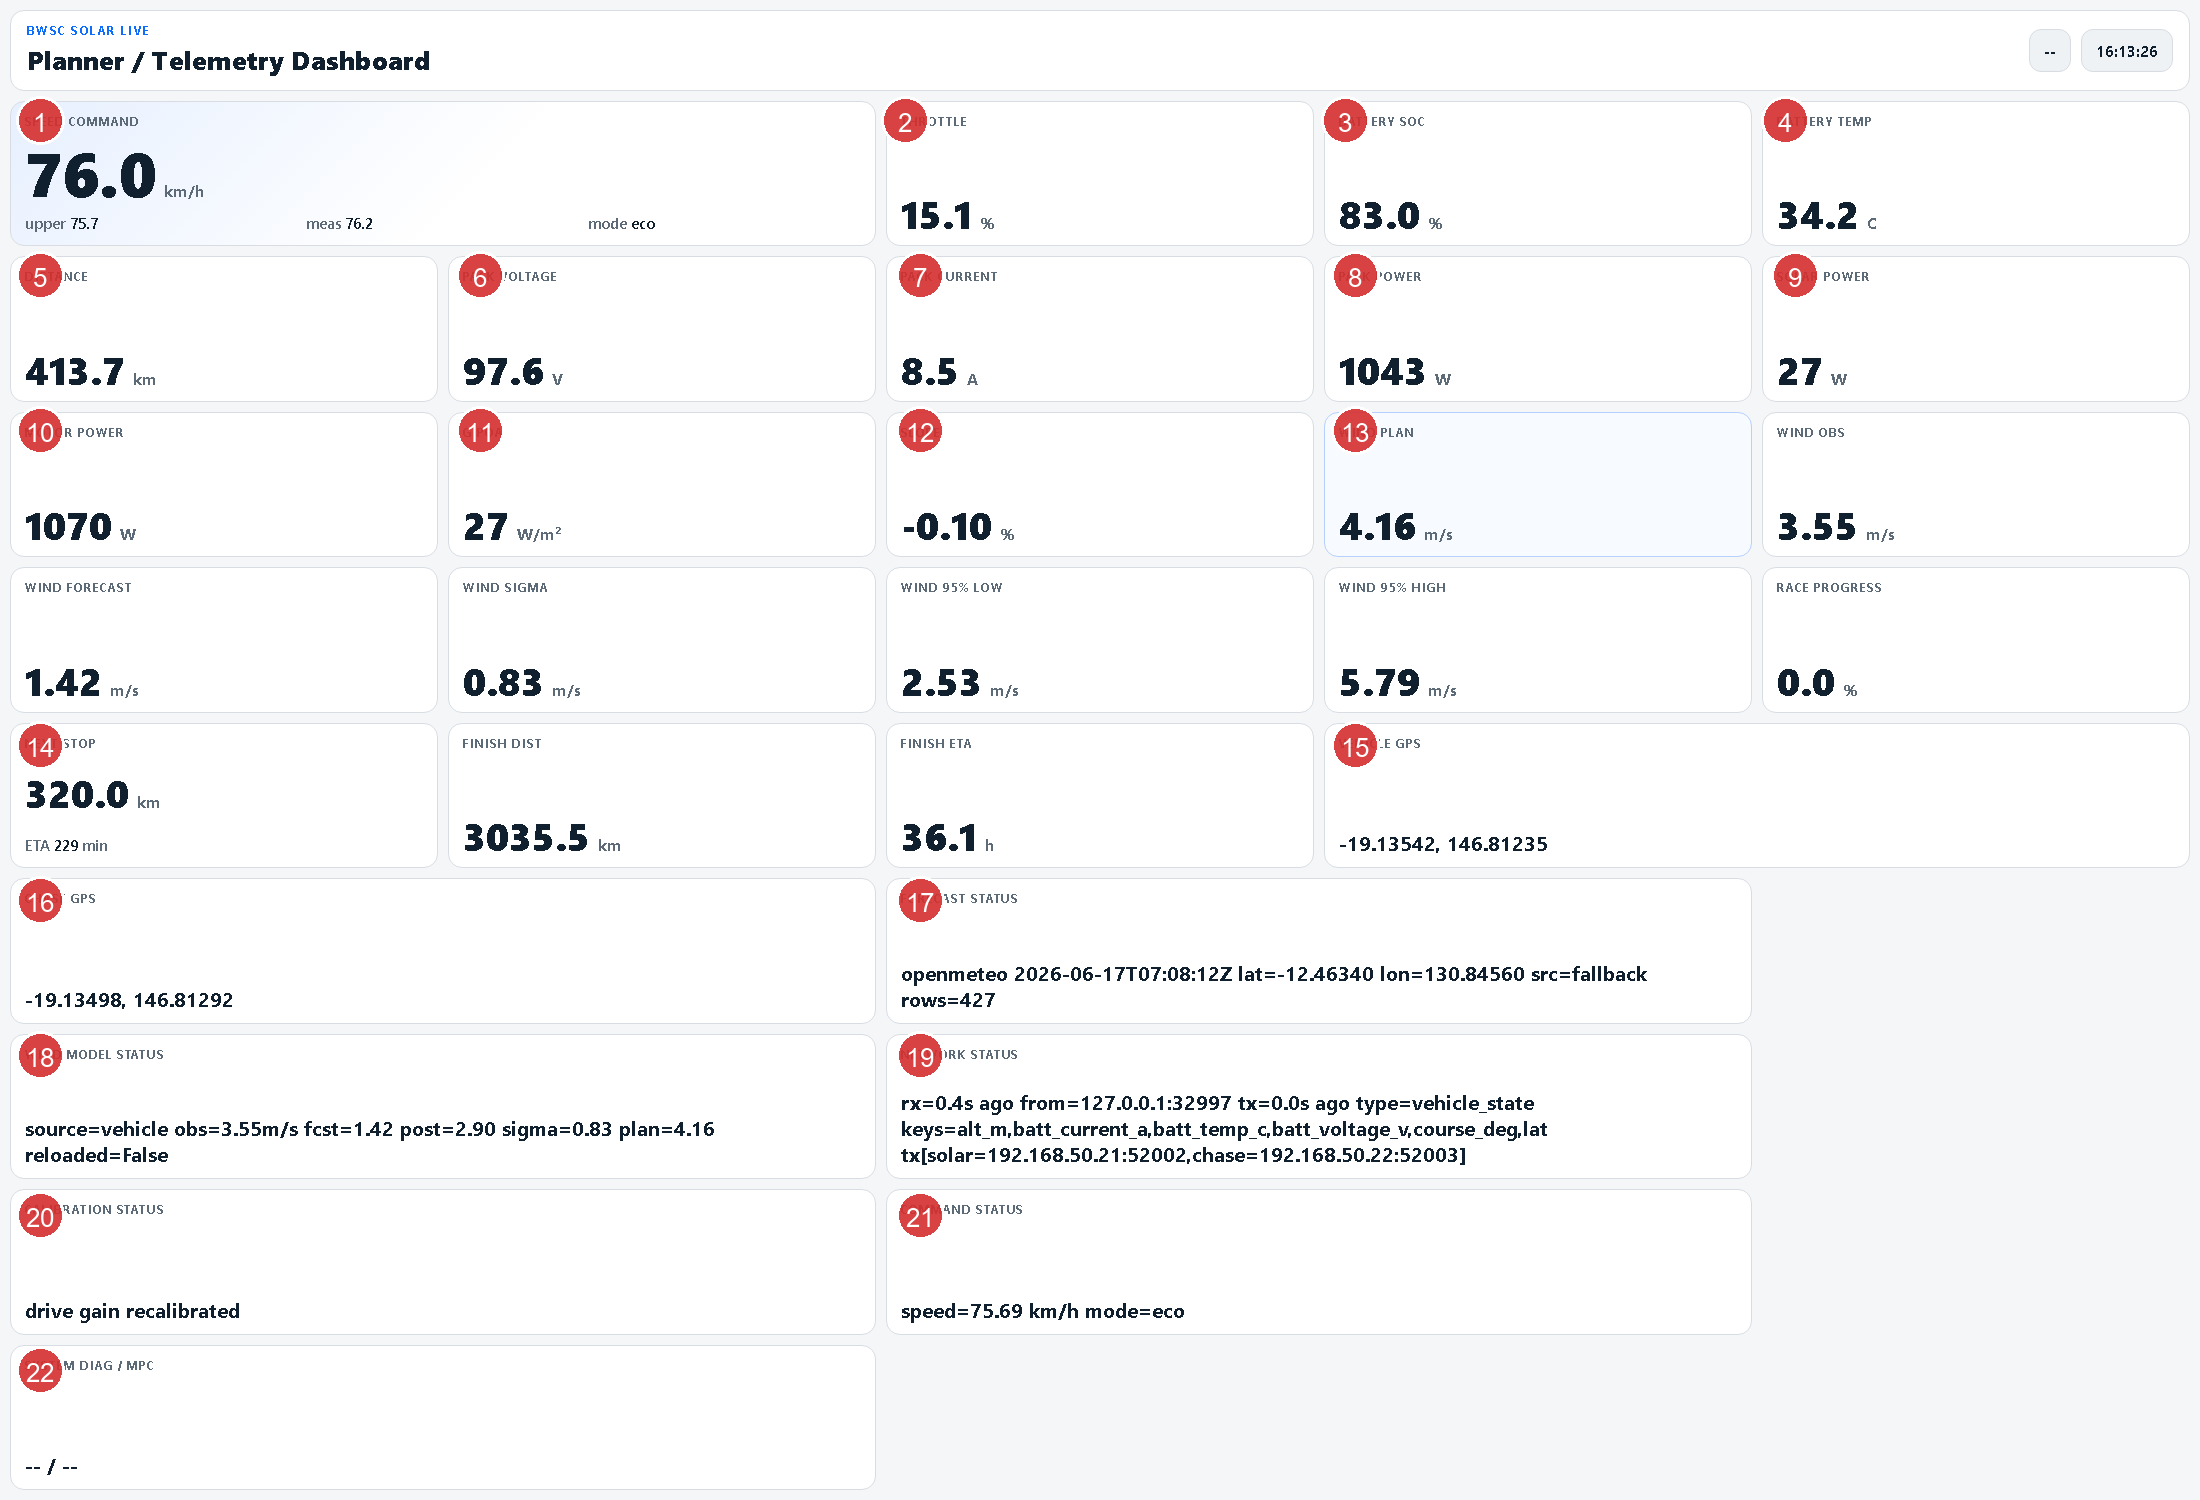
\includegraphics[width=0.98\linewidth]{assets/dashboard_live_wifi_annotated.png}
\end{center}
\end{landscape}

\clearpage
\begin{landscape}
\section*{dashboard 上半分拡大}
\begin{center}
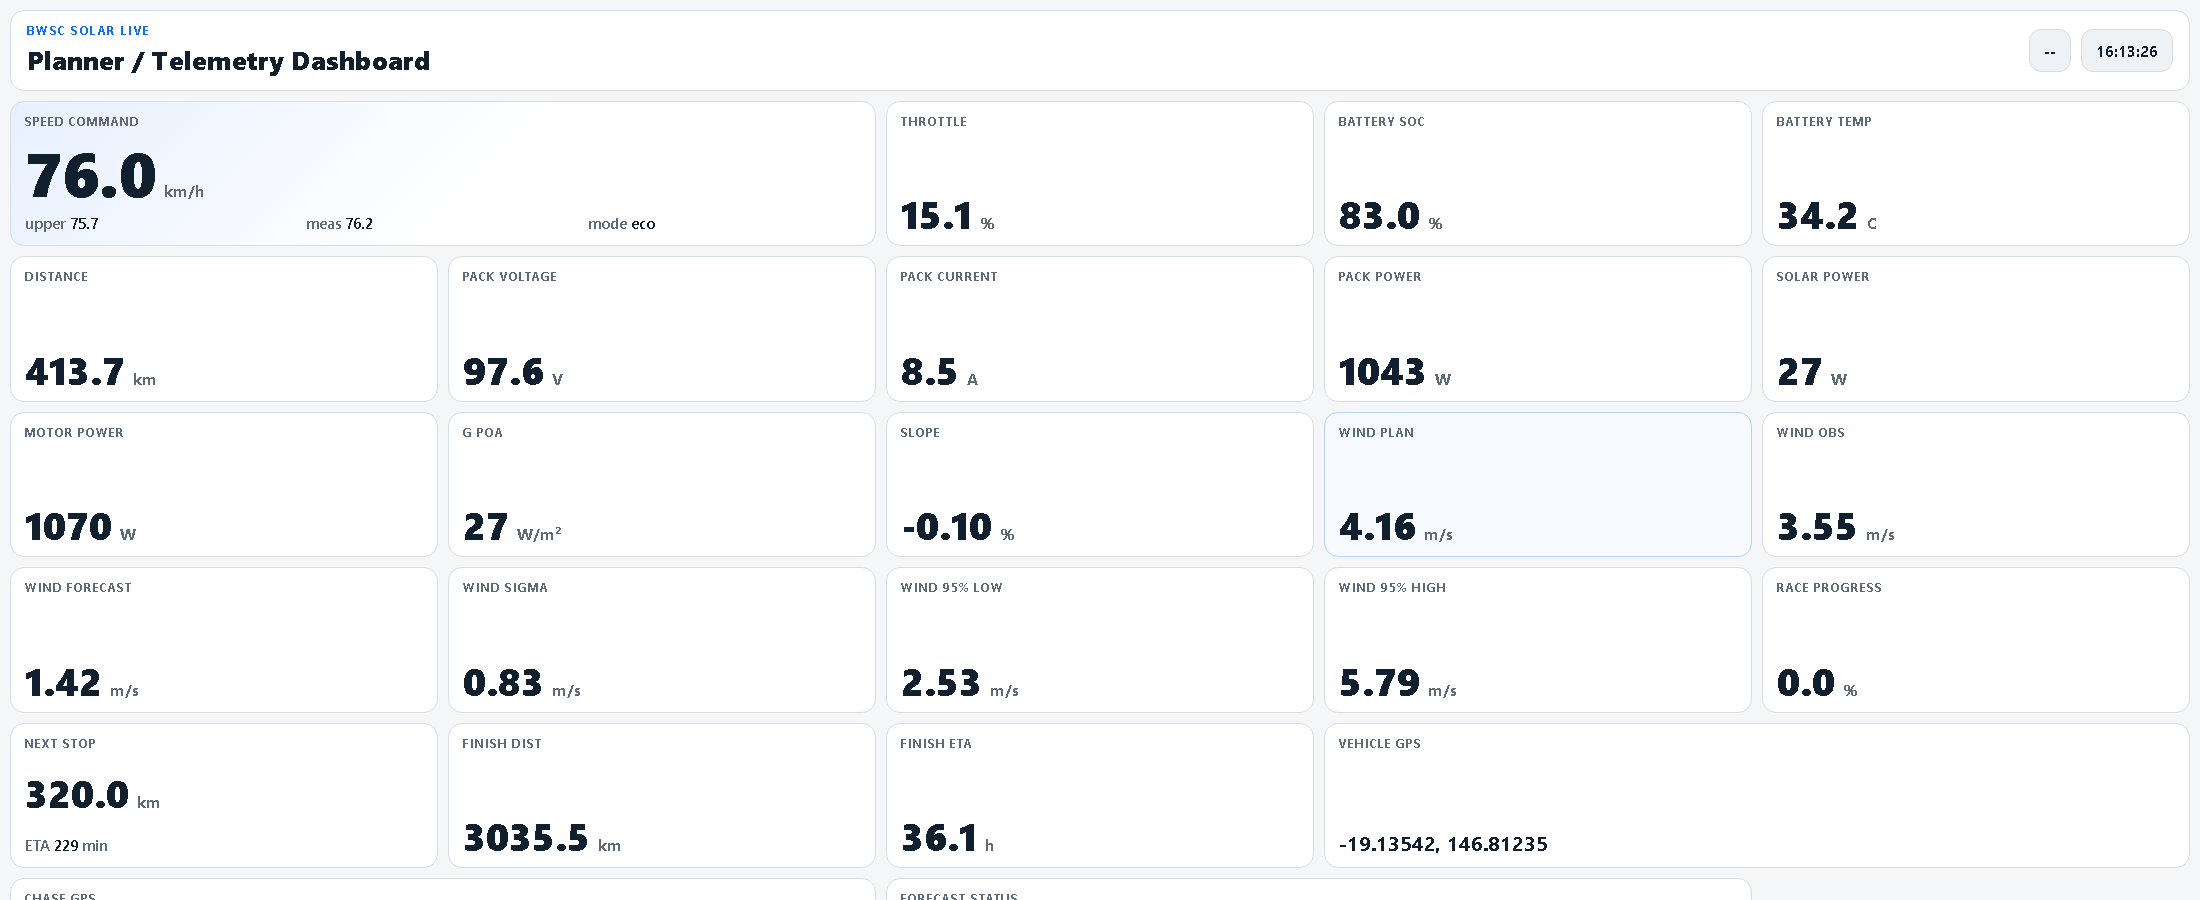
\includegraphics[width=0.98\linewidth]{assets/dashboard_live_wifi_top.png}
\end{center}
\end{landscape}

\clearpage
\begin{landscape}
\section*{dashboard 下半分拡大}
\begin{center}
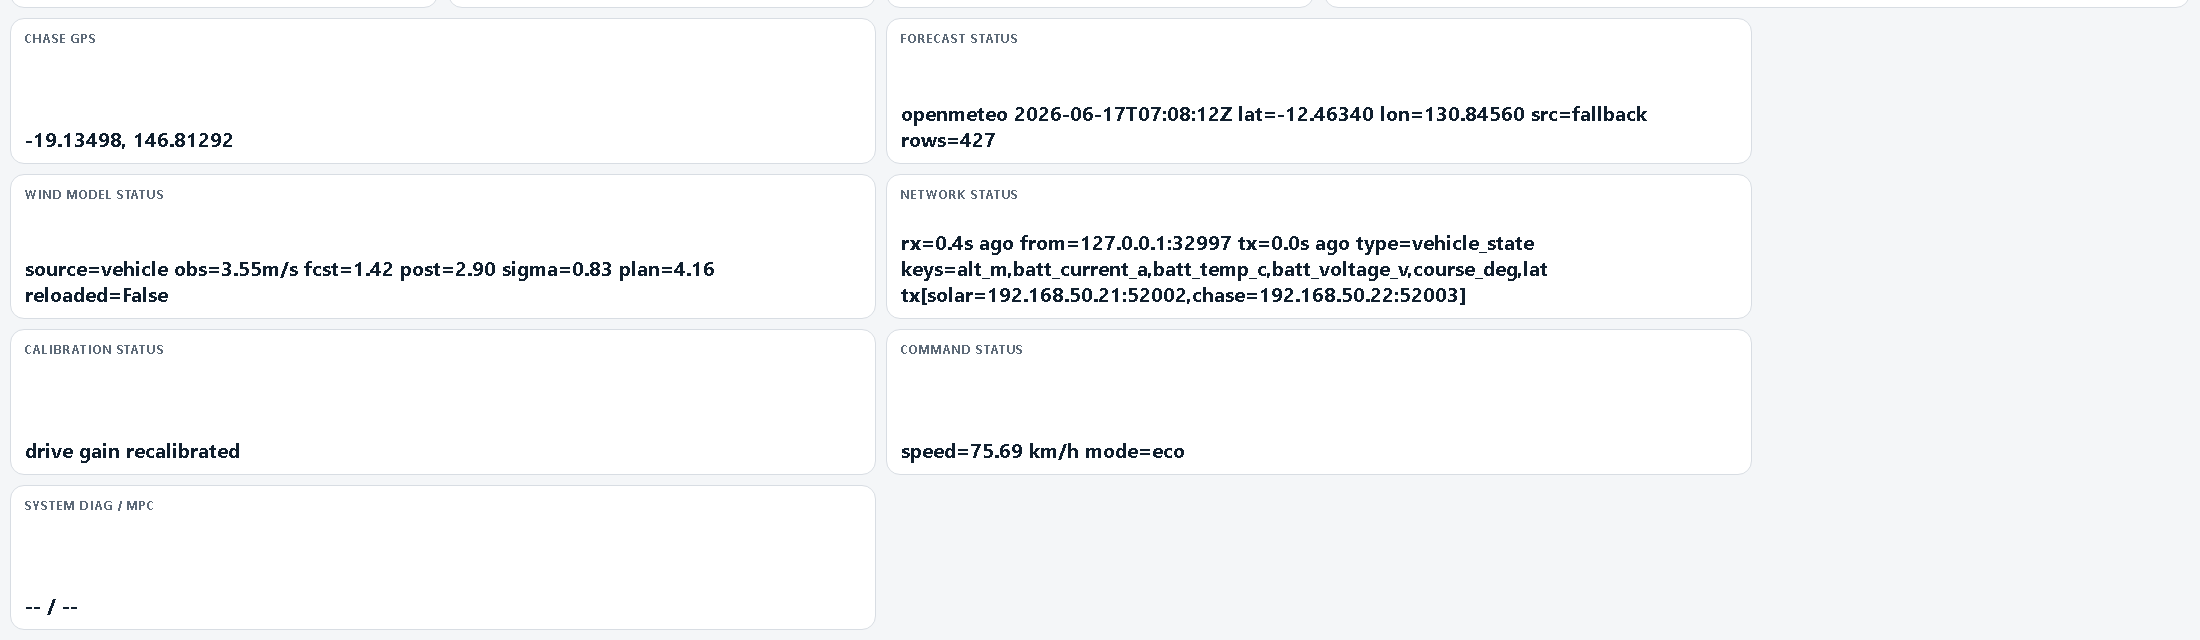
\includegraphics[width=0.98\linewidth]{assets/dashboard_live_wifi_bottom.png}
\end{center}
\end{landscape}

\clearpage
\section{番号ごとの説明}

\begin{longtable}{p{0.06\linewidth}p{0.16\linewidth}p{0.27\linewidth}p{0.22\linewidth}p{0.21\linewidth}}
\toprule
No. & 表示 & 何を表すか & 正常時の見方 & 異常/注意時の行動 \\
\midrule
\endhead
1 & Speed Command & 下位 planner が車両へ出した速度司令 & \path{upper}, \path{meas}, \path{mode} と合わせて見る & \path{meas} が追従しないなら車両側追従不良または clamp を疑う \\
2 & Throttle & planner が計算した下位入力 & 高いほど駆動要求が大きい & 100\% 張り付きなら上位要求過大か車両追従不足 \\
3 & Battery SoC & バッテリ残量 & 目標 SoC に対して十分かを見る & 急減時は speed command を下げる判断材料 \\
4 & Battery Temp & 電池温度 & 運用温度帯か確認 & 上昇しすぎなら保護・制限を検討 \\
5 & Distance & 現在地点の route 距離 \path{s_km} & next stop / finish と整合しているか & 不自然なら GPS / distance node を確認 \\
6 & Pack Voltage & パック電圧 & SoC や負荷と整合しているか & 急低下なら負荷過大や電池異常を疑う \\
7 & Pack Current & パック電流 & 消費傾向の把握 & 高止まりなら過大消費を疑う \\
8 & Pack Power & パック電力 & 実質的な電池出力 & 想定以上なら speed / slope / headwind を確認 \\
9 & Solar Power & 太陽から入っている電力 & 日射と整合するか & 低すぎるなら雲・角度・センサ・パネル異常候補 \\
10 & Motor Power & 駆動電力 & Pack Power と比較して損失感を掴む & 急上昇なら速度指令や勾配を確認 \\
11 & G POA & パネル面入射日射 & solar power の説明変数 & \path{src=fallback} 中は forecast 依存であることに注意 \\
12 & Slope & 現在勾配 & 負荷増減の説明に使う & 不自然なら GPS / altitude / route profile を確認 \\
13 & Wind Block & \path{Wind Plan}, \path{Obs}, \path{Forecast}, \path{Sigma}, 95\% 区間のまとまり & planner が何を想定し、どれくらい不確かかを見る & \path{Obs} と \path{Forecast} がズレ続けるなら tuning 見直し \\
14 & Next Stop / Finish & 次 stop までの距離と ETA、finish 残距離/ETA & 戦略判断の中心 & ETA が崩れたら上位プラン再確認 \\
15 & Vehicle GPS & ソーラーカー位置 & route 上の現在地確認 & 空欄なら車両送信が来ていない \\
16 & Chase GPS & 伴走車位置 & 伴走車の計測基準確認 & 空欄なら chase sender を確認 \\
17 & Forecast Status & weather node の取得状態 & \path{src=gps} が理想、rows も確認 & \path{src=fallback} のまま本番運用しない \\
18 & Wind Model Status & 風補正の現在状態 & \path{source=vehicle/chase}, \path{obs}, \path{fcst}, \path{post}, \path{sigma}, \path{plan} を読む & \path{waiting observation} なら風入力が来ていない \\
19 & Network Status & 通信の鮮度と送信元 & \path{rx=0.xs ago} が理想 & \path{rx=never} や数秒更新なしなら通信断 \\
20 & Calibration Status & 自動校正の進行状態 & \path{collecting} は起動直後に自然 & 異常な補正が続くなら log を見直す \\
21 & Command Status & 再配信された車両 command の要約 & speed と mode が出ていれば正常 & 出ないなら command bridge を確認 \\
22 & System Diag / MPC & 予備の診断欄 & 将来の診断表示枠 & 値が入るよう拡張可能 \\
\bottomrule
\end{longtable}

\subsection{dashboard で最優先で見るべき 6 項目}

\begin{enumerate}
  \item \path{Speed Command}
  \item \path{Battery SoC}
  \item \path{Wind Plan}
  \item \path{Next Stop}
  \item \path{Network Status}
  \item \path{Forecast Status}
\end{enumerate}

\subsection[-- が出る意味]{\texttt{--} が出る意味}

\path{--} は主に次を意味する。

\begin{itemize}
  \item topic がまだ来ていない
  \item sender 側がその field を送っていない
  \item live mode では未使用
  \item node が未計算
\end{itemize}

本番運用で \path{--} のままにしてよいものと、だめなもの:

\begin{longtable}{p{0.28\linewidth}p{0.18\linewidth}}
\toprule
項目 & \path{--} 許容か \\
\midrule
\endhead
Speed Command & 不可 \\
Battery SoC & 不可 \\
Vehicle GPS & 不可 \\
Network Status & 不可 \\
Forecast Status & 不可 \\
Wind Model Status & 通常は不可 \\
System Diag / MPC & 可 \\
\bottomrule
\end{longtable}

\section{典型的な異常と対処}

\begin{longtable}{p{0.28\linewidth}p{0.28\linewidth}p{0.28\linewidth}}
\toprule
症状 & まず疑うこと & すぐやること \\
\midrule
\endhead
\path{network status} が \path{rx=never} & sender 不起動、port 違い、WiFi 断 & Pi 側 sender と IP/port を確認 \\
\path{forecast status} が \path{src=fallback} のまま & chase GPS 未受信 & chase sender を確認 \\
\path{wind model waiting observation} & wind field 未送信 & \path{wind_speed_ms}, \path{wind_dir_deg}, \path{course_deg} を確認 \\
\path{meas} が \path{speed command} に追従しない & 車両制御側問題、safety clamp & 車両 firmware と actual speed を確認 \\
SoC が急減 & 消費過大、風、勾配、電池異常 & speed command を見直し、電池電圧/電流確認 \\
distance が止まる & GPS / speed topic 欠損 & \path{/vehicle/speed_kmh} と \path{/vehicle/s_km} 確認 \\
command は出るが車両が動かない & receiver 実装不足 & マイコン受信ログと clamp 条件確認 \\
\bottomrule
\end{longtable}

\section{チーム引き継ぎの受け入れ基準}

この資料を使った引き継ぎが完了したと判断する条件:

\begin{enumerate}
  \item 新メンバーが \path{simulate} を単独実行できる
  \item 新メンバーが \path{measure up} を単独実行できる
  \item 新メンバーが \path{live_wifi up} を単独実行できる
  \item 新メンバーが dashboard の主要 10 項目を説明できる
  \item 新メンバーが sender JSON の必須 field を説明できる
  \item 新メンバーが \path{route}, \path{weather}, \path{stop}, \path{maps} の差し替え場所を知っている
  \item 新メンバーが sample のままなものを列挙できる
\end{enumerate}

\section{運用開始前に必ず更新すべきファイル}

\begin{itemize}
  \item \path{config/solar/bwsc_2027_demo.yaml}
  \item \path{data/route/bwsc_route_waypoints_*.csv}
  \item \path{data/route/bwsc_route_profile_*.csv}
  \item \path{data/route/bwsc_speed_profile_*.csv}
  \item \path{data/race/bwsc_control_stops_*.yaml}
  \item \path{data/weather/*.csv} または live forecast 方針
  \item \path{maps/*.csv}
  \item Pi / ESP32 の sender / receiver 実装
\end{itemize}

\section{この資料と併用する文書}

\begin{itemize}
  \item \path{docs/solar_workflow.pdf}
  \item \path{docs/solar_live_wifi_manual.pdf}
  \item \path{rqt_graph_solar_live_wifi.png}
  \item BWSC official regulations
  \item BWSC Team Manager's Guide
  \item 2027 route notes
\end{itemize}

\section{最終メッセージ}

このパッケージは、\textbf{そのまま魔法のように勝手に正解を出すものではない}。
強いのは次の 3 点である。

\begin{enumerate}
  \item 情報を 1 か所に集めて見える化できること
  \item シミュレーションと本番を同じ設計思想で回せること
  \item 実測を次回改善へ戻せること
\end{enumerate}

逆に、最終的な勝負を決めるのは次である。

\begin{itemize}
  \item route / stop / weather の入力品質
  \item vehicle model と map の品質
  \item 通信実装の安定性
  \item チームが dashboard を読んで判断できること
\end{itemize}

この文書を使って、\textbf{全員が「自分でも動かせる」と言える状態}まで持っていってほしい。

\end{document}
